\section{Phát biểu bài toán và hai pipeline của hệ thống}

\subsection{Đầu vào và đầu ra của bài toán}

Nghiên cứu xem xét bài toán hỏi--đáp y khoa tin cậy dựa trên kiến trúc truy xuất tăng cường sinh nội dung (Retrieval-Augmented Generation, RAG) \cite{lewis2020}. Hệ thống kết hợp tri thức y khoa đã được kiểm chứng với mô hình ngôn ngữ lớn (Large Language Model, LLM), qua đó ưu tiên bằng chứng truy xuất thay vì chỉ dựa vào tri thức được ghi nhớ trong tham số mô hình.

Trong giai đoạn huấn luyện, đầu vào thứ nhất là tập tài liệu y khoa đã được kiểm chứng
\[
    D = \{d_1,d_2,\ldots,d_{N_D}\},
\]
trong đó $d_j$ là tài liệu thứ $j$ và $N_D$ là số tài liệu. Tập $D$ có thể bao gồm giáo trình, hướng dẫn lâm sàng, phác đồ chẩn đoán--điều trị và các cặp hỏi--đáp đã được chuyên gia xác nhận. Đầu vào thứ hai là bộ dữ liệu hỏi--đáp
\[
    \mathcal{T}_{\mathrm{QA}}
    = \{(q_i,u_i,h_i,y_i^*)\}_{i=1}^{N_Q},
\]
trong đó $N_Q$ là số mẫu huấn luyện; $q_i$ là câu hỏi y khoa; $u_i$ là phần bối cảnh bệnh nhân được phép sử dụng; $h_i$ là lịch sử hội thoại; và $y_i^*$ là câu trả lời chuẩn của mẫu thứ $i$.

Sau tiền xử lý, tập tài liệu $D$ được phân chia thành tập các đoạn văn bản
\[
    C = \{c_1,c_2,\ldots,c_{N_C}\},
\]
trong đó $c_j$ là một đoạn văn bản (chunk) và $N_C$ là tổng số đoạn. Các đoạn cùng siêu dữ liệu và biểu diễn tìm kiếm được lưu trong chỉ mục tri thức $I$. Với mỗi mẫu hỏi--đáp, hệ thống truy xuất tập bằng chứng $C_i^* \subseteq C$ để hình thành mẫu tinh chỉnh $(q_i,u_i,h_i,C_i^*,y_i^*)$.

Trong giai đoạn suy diễn, đầu vào của một lượt hỏi được biểu diễn bởi
\[
    X=(q,u,h,I),
\]
trong đó $q$ là câu hỏi hiện tại, $u$ là bối cảnh bệnh nhân cần thiết và được phép sử dụng, $h$ là lịch sử hội thoại, còn $I$ là chỉ mục tri thức đã được xây dựng từ tập tài liệu $D$.

Đầu ra chính không chỉ là một câu trả lời mà là cặp
\[
    O=(\hat{y},d),
    \qquad
    d\in\Delta=\{\text{Answer},\text{Abstain},\text{Escalate}\},
\]
trong đó $\hat{y}$ là phản hồi cuối cùng và $d$ là quyết định thuộc tập hành động $\Delta$. Quyết định \emph{Answer} được chọn khi bằng chứng đủ mạnh và câu trả lời an toàn; \emph{Abstain} biểu thị việc từ chối trả lời khi bằng chứng thiếu, mâu thuẫn hoặc độ tin cậy thấp; còn \emph{Escalate} chuyển người dùng đến bác sĩ hoặc chuyên gia khi tình huống có nguy cơ cao, khẩn cấp hay vượt phạm vi của hệ thống. Khi phù hợp, đầu ra còn kèm các đoạn bằng chứng, nguồn trích dẫn, độ tin cậy và cảnh báo an toàn.

\subsection{Các tham số cần học và biến trung gian}

Các ẩn cần tìm của bài toán được chia thành hai nhóm. Nhóm thứ nhất là bộ tham số được học hoặc hiệu chỉnh trong giai đoạn huấn luyện:
\[
    \Theta=\{\phi,\theta,\psi\},
\]
trong đó $\phi$ là tham số của bộ truy xuất, quyết định cách biểu diễn và chấm điểm độ liên quan giữa truy vấn với đoạn tài liệu; $\theta$ là tham số của LLM dùng để sinh câu trả lời; và $\psi$ là tham số cùng các ngưỡng của lớp bảo đảm chất lượng, dùng để đánh giá bằng chứng, độ an toàn và lựa chọn quyết định cuối cùng.

Nhóm thứ hai gồm các biến phải suy ra cho mỗi lượt hỏi:
\begin{itemize}
    \item $q'$: truy vấn độc lập đã được chuẩn hóa từ câu hỏi hiện tại và ngữ cảnh liên quan;
    \item $m$ và $e$: lần lượt là ý định y khoa và tập thực thể y khoa được nhận diện trong truy vấn;
    \item $\mathbf{z}_q\in\mathbb{R}^{d_e}$: vector nhúng $d_e$ chiều của truy vấn;
    \item $C^*=\{c_{(1)},\ldots,c_{(k)}\}\subseteq C$: tập $k$ đoạn bằng chứng liên quan nhất;
    \item $\widetilde{y}$: câu trả lời nháp do LLM sinh ra;
    \item $\mathbf{v}$: vector điểm chất lượng gồm độ liên quan, độ bám sát bằng chứng, tính đầy đủ, độ chính xác trích dẫn, độ an toàn và độ tin cậy;
    \item $d\in\Delta$: quyết định cuối cùng của hệ thống.
\end{itemize}

\subsection{Nguyên lý và phát biểu toán học tổng quát}

Nguyên lý cốt lõi của bài toán là sinh phản hồi có căn cứ và có chọn lọc. Bộ truy xuất cung cấp bằng chứng từ kho tri thức đã kiểm chứng; LLM tổng hợp câu trả lời trên bằng chứng đó; lớp bảo đảm chất lượng có quyền ngăn câu trả lời hoặc chuyển đến chuyên gia khi điều kiện an toàn không được đáp ứng. Toàn bộ bài toán được biểu diễn bởi ánh xạ
\[
    F_{\phi,\theta,\psi}:(q,u,h,I)\longrightarrow(C^*,\hat{y},d).
\]
Trong đó, các thành phần đầu vào, đầu ra và tham số đã được định nghĩa ở hai mục trên. Gọi $\mathcal{T}$ là phân phối dữ liệu đánh giá và $\mathcal{U}$ là hàm hữu dụng y khoa phản ánh đồng thời độ chính xác, độ bám sát bằng chứng, độ an toàn và chất lượng quyết định. Bài toán tối ưu tổng quát là
\[
    (\phi^*,\theta^*,\psi^*)
    =\arg\max_{\phi,\theta,\psi}
    \mathbb{E}_{X\sim\mathcal{T}}
    \left[\mathcal{U}\bigl(F_{\phi,\theta,\psi}(X)\bigr)\right].
\]
Việc tối ưu phải thỏa mãn các ràng buộc về thời gian phản hồi, bộ nhớ và độ dài cửa sổ ngữ cảnh. Các phép biến đổi cụ thể tạo nên ánh xạ $F_{\phi,\theta,\psi}$ được trình bày trong hai pipeline dưới đây.

\subsection{Pipeline huấn luyện}

Pipeline huấn luyện tạo kho tri thức có thể truy xuất, dữ liệu tinh chỉnh RAG, LLM chuyên biệt và các ngưỡng chất lượng--an toàn. Tổng quan pipeline được trình bày trong Hình~\ref{fig:training-pipeline}; quy trình gồm năm bước sau.

\begin{figure}[htbp]
    \centering
    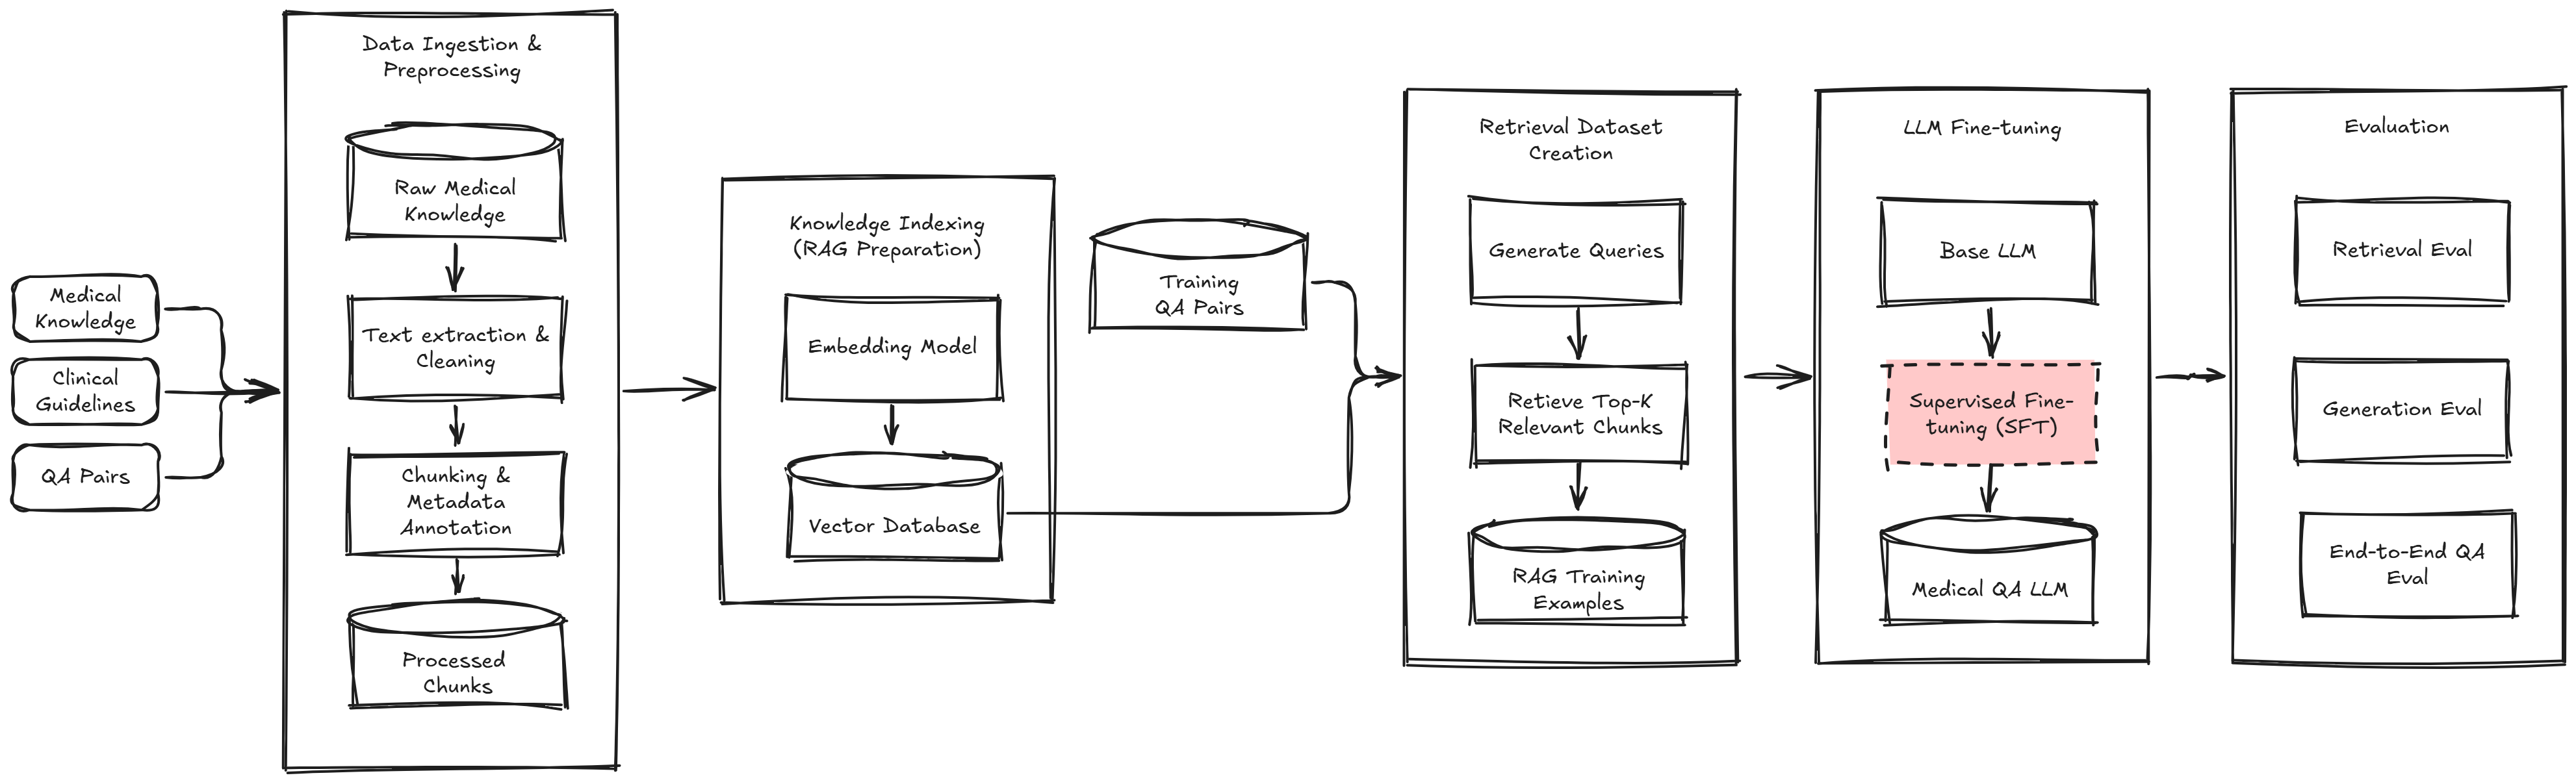
\includegraphics[width=\textwidth]{img/training_pipeline.png}
    \caption{Pipeline huấn luyện của hệ thống hỏi--đáp y khoa dựa trên RAG}
    \label{fig:training-pipeline}
\end{figure}

\subsubsection{Bước 1: Thu thập và tiền xử lý dữ liệu}

Tập tài liệu $D$ được thu thập từ các nguồn y khoa chính thống như giáo trình, hướng dẫn lâm sàng, phác đồ chẩn đoán--điều trị và các cặp hỏi--đáp đã được kiểm chứng. Tài liệu thô ở dạng PDF, Word, HTML hoặc cơ sở dữ liệu được trích xuất văn bản; loại bỏ đầu trang, chân trang, ký tự lỗi và nội dung trùng lặp; chuẩn hóa thuật ngữ, đơn vị và định dạng; đồng thời loại bỏ hoặc ẩn thông tin nhận dạng bệnh nhân.

Hàm phân đoạn $f_{\mathrm{chunk}}$ chuyển tập tài liệu thành các đoạn:
\[
    C=f_{\mathrm{chunk}}(D;\ell,s),
\]
trong đó $\ell$ là kích thước đoạn và $s$ là bước trượt. Mỗi đoạn $c_j$ được gắn siêu dữ liệu $\mu_j$ gồm tên tài liệu, chuyên khoa, chủ đề, tổ chức phát hành, ngày ban hành, phiên bản, vị trí trong tài liệu, phạm vi áp dụng, trạng thái hiệu lực và độ tin cậy của nguồn. Đầu ra của bước này là tập các đoạn sạch $(c_j,\mu_j)$ đủ thông tin để truy xuất và trích dẫn.

\subsubsection{Bước 2: Lập chỉ mục tri thức và huấn luyện bộ truy xuất}

Mô hình nhúng $E_{\phi}$ biến mỗi đoạn $c_j$ thành vector $\mathbf{z}_j=E_{\phi}(c_j)\in\mathbb{R}^{d_e}$. Vector, nội dung đoạn, siêu dữ liệu và thông tin trích dẫn được lưu trong chỉ mục đặc $I_{\mathrm{dense}}$; đồng thời, biểu diễn từ khóa được lưu trong chỉ mục thưa $I_{\mathrm{sparse}}$. Chỉ mục tri thức hoàn chỉnh là $I=(I_{\mathrm{dense}},I_{\mathrm{sparse}})$.

Điểm truy xuất lai giữa truy vấn $q$ và đoạn $c$ được xác định bởi
\[
    s_{\phi}(q,c)
    =\alpha s_{\mathrm{dense},\phi}(q,c)
    +(1-\alpha)s_{\mathrm{sparse}}(q,c),
\]
trong đó $s_{\mathrm{dense},\phi}$ là điểm tương đồng ngữ nghĩa, $s_{\mathrm{sparse}}$ là điểm khớp từ khóa và $\alpha\in[0,1]$ là hệ số phối hợp hai thành phần.

Khi có nhãn đoạn dương và đoạn âm, bộ truy xuất được huấn luyện để đưa câu hỏi gần đoạn liên quan và xa các đoạn không liên quan. Với $c_i^+$ là đoạn đúng và $\mathcal{B}_i^-$ là tập đoạn âm hoặc âm khó của câu hỏi $q_i$, hàm mất mát truy xuất được xác định bởi \cite{karpukhin2020}
\[
    \mathcal{L}_{\mathrm{ret}}(\phi)
    =-\sum_i\log
    \frac{\exp(s_{\phi}(q_i,c_i^+))}
    {\exp(s_{\phi}(q_i,c_i^+))+
     \sum_{c^-\in\mathcal{B}_i^-}\exp(s_{\phi}(q_i,c^-))}.
\]
Nếu tham số $\phi$ được cập nhật, toàn bộ vector đoạn phải được tạo lại và chỉ mục $I_{\mathrm{dense}}$ phải được cập nhật trước các bước tiếp theo.

\subsubsection{Bước 3: Tạo dữ liệu huấn luyện RAG}

Từ bộ $\mathcal{T}_{\mathrm{QA}}$, câu hỏi được chuẩn hóa hoặc mở rộng bằng các cách diễn đạt tương đương, câu hỏi sinh từ tài liệu, câu hỏi nối tiếp trong hội thoại và trường hợp cố ý thiếu bằng chứng. Với mỗi câu hỏi, hệ thống thực hiện truy xuất lai, lấy Top-$k$ đoạn, lọc theo siêu dữ liệu và có thể xếp hạng lại để thu được $C_i^*$.

Tập mẫu tinh chỉnh được tạo thành
\[
    \mathcal{T}_{\mathrm{RAG}}
    =\{(q_i,u_i,\bar{h}_i,C_i^*,y_i^*,d_i^*)\}_{i=1}^{N_Q},
\]
trong đó $\bar{h}_i$ là lịch sử đã cô đọng và $d_i^*\in\Delta$ là nhãn hành động chuẩn. Mỗi mẫu dạy mô hình đọc bằng chứng, trả lời dựa trên nguồn, trích dẫn đúng, biểu đạt độ không chắc chắn, từ chối khi bằng chứng không đủ và chuyển chuyên gia đối với tình huống nguy cơ cao.

\subsubsection{Bước 4: Tinh chỉnh LLM và lớp quyết định}

LLM nền được tinh chỉnh có giám sát (Supervised Fine-Tuning, SFT) trên $\mathcal{T}_{\mathrm{RAG}}$. Hàm mất mát sinh câu trả lời là
\[
    \mathcal{L}_{\mathrm{gen}}(\theta)
    =-\sum_i\sum_{t=1}^{T_i}
    \log P_{\theta}\!\left(
        y_{i,t}^*\mid y_{i,<t}^*,q_i,u_i,\bar{h}_i,C_i^*
    \right),
\]
trong đó $T_i$ là độ dài câu trả lời chuẩn và $y_{i,<t}^*$ là các token đứng trước vị trí $t$. Lớp bảo đảm chất lượng được học hoặc hiệu chỉnh bằng hàm mất mát $\mathcal{L}_{\mathrm{safe}}(\psi)$, bao gồm lỗi phân loại quyết định $d_i^*$ và các lỗi liên quan đến độ bám sát bằng chứng, trích dẫn và an toàn.

Hàm mục tiêu tổng hợp được viết dưới dạng
\[
    \mathcal{L}
    =\lambda_{\mathrm{ret}}\mathcal{L}_{\mathrm{ret}}
    +\lambda_{\mathrm{gen}}\mathcal{L}_{\mathrm{gen}}
    +\lambda_{\mathrm{safe}}\mathcal{L}_{\mathrm{safe}},
\]
trong đó các hệ số không âm $\lambda_{\mathrm{ret}}$, $\lambda_{\mathrm{gen}}$ và $\lambda_{\mathrm{safe}}$ kiểm soát đóng góp tương đối của ba mục tiêu. Các thành phần có thể được tối ưu theo từng giai đoạn, nhưng phải được đánh giá lại trong cùng một pipeline đầu cuối.

\subsubsection{Bước 5: Đánh giá và lựa chọn mô hình}

Đánh giá được thực hiện ở ba tầng:
\begin{itemize}
    \item \textbf{Tầng truy xuất:} sử dụng $\mathrm{Recall}@k$, $\mathrm{Precision}@k$, Mean Reciprocal Rank (MRR), normalized Discounted Cumulative Gain (nDCG) và tỷ lệ tài liệu chuẩn xuất hiện trong Top-$k$ để kiểm tra khả năng tìm đúng bằng chứng \cite{xiong2024mirage}.
    \item \textbf{Tầng sinh câu trả lời:} đánh giá độ chính xác y khoa, độ liên quan, độ trung thực và bám sát bằng chứng, tính đầy đủ, tỷ lệ ảo giác, độ chính xác của trích dẫn và độ an toàn \cite{ragas2023, medtrustrag}.
    \item \textbf{Tầng hỏi--đáp đầu cuối:} đánh giá toàn bộ chuỗi từ câu hỏi, truy xuất, xây dựng câu lệnh, sinh câu trả lời, kiểm tra chất lượng đến quyết định cuối cùng; trong đó kiểm tra riêng khả năng trả lời đúng, từ chối đúng và chuyển chuyên gia đúng.
\end{itemize}

Đầu ra của pipeline huấn luyện gồm chỉ mục tri thức $I$, tập mẫu $\mathcal{T}_{\mathrm{RAG}}$, LLM hỏi--đáp y khoa đã tinh chỉnh, tham số hoặc ngưỡng chất lượng--an toàn $\psi$, kết quả đánh giá và checkpoint mô hình tốt nhất.

\subsection{Pipeline suy diễn}

Pipeline suy diễn sử dụng các thành phần đã tạo trong huấn luyện để xử lý một lượt hỏi qua năm bước. Luồng xử lý từ đầu vào đến quyết định Answer--Abstain--Escalate được minh họa trong Hình~\ref{fig:inference-pipeline}.

\begin{figure}[htbp]
    \centering
    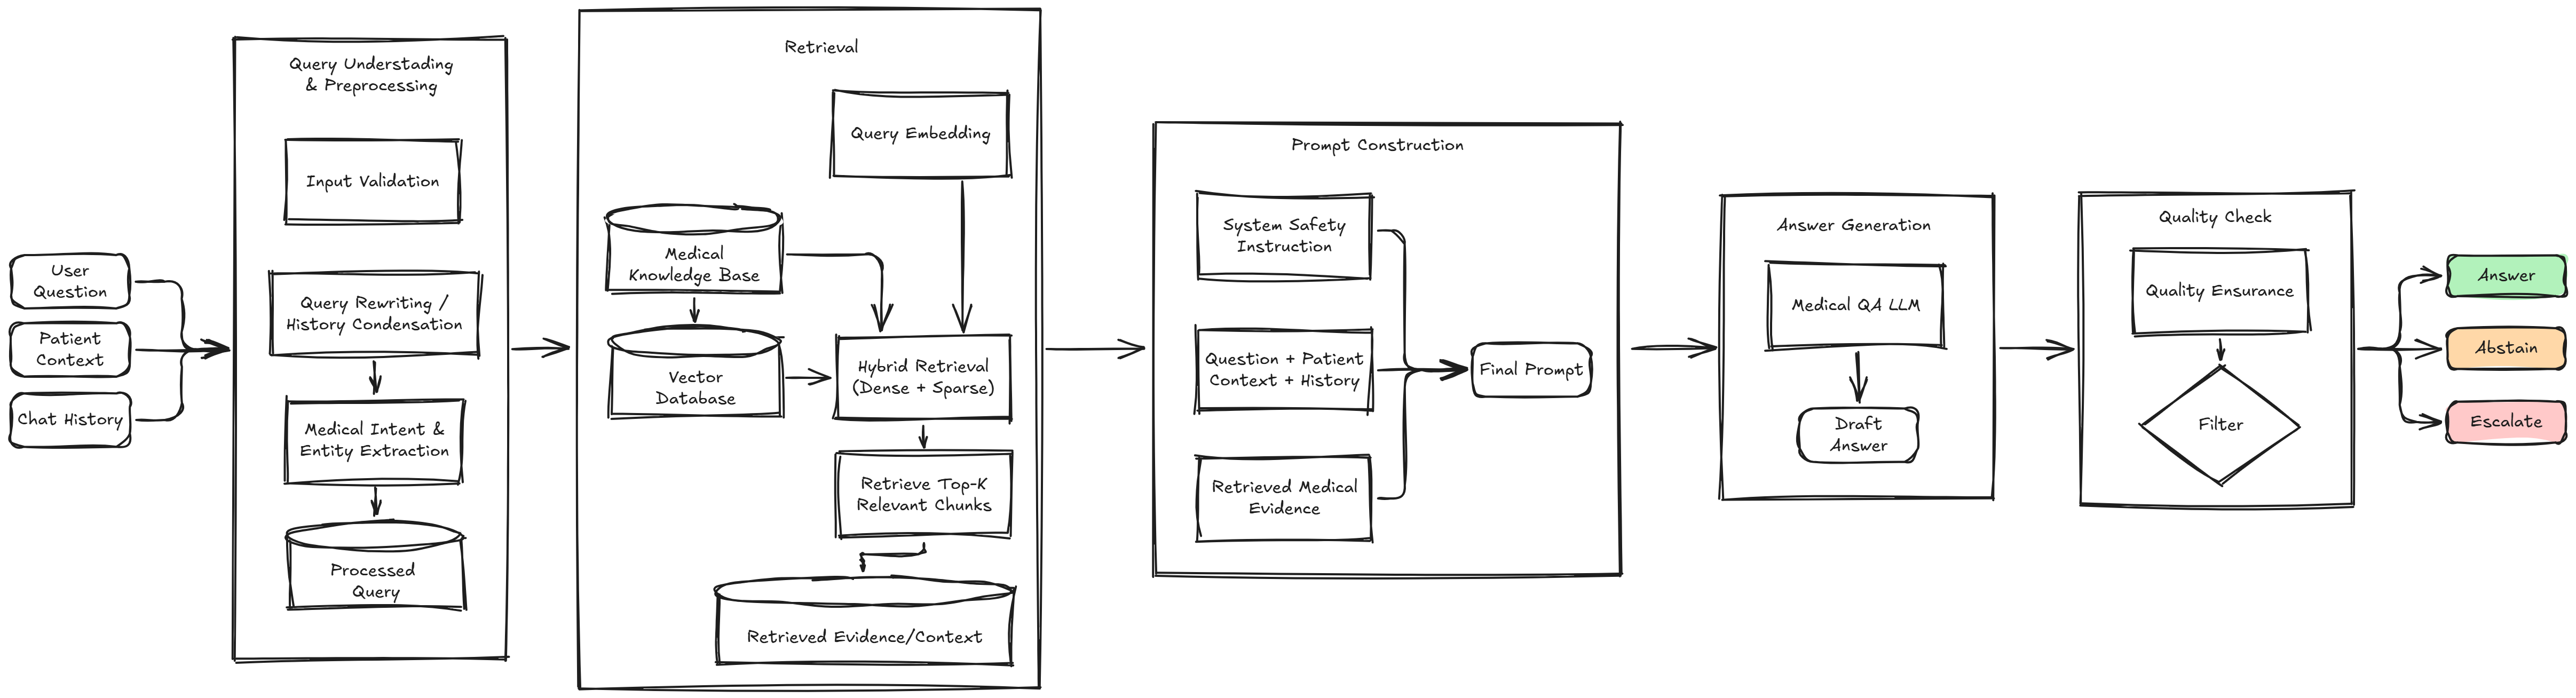
\includegraphics[width=\textwidth]{img/infer_pipeline.png}
    \caption{Pipeline suy diễn và cơ chế quyết định phản hồi của hệ thống}
    \label{fig:inference-pipeline}
\end{figure}

\subsubsection{Bước 1: Hiểu và tiền xử lý truy vấn}

Hệ thống tiếp nhận câu hỏi $q$, bối cảnh bệnh nhân $u$ và lịch sử hội thoại $h$. Bối cảnh bệnh nhân có thể gồm tuổi, giới tính, triệu chứng, tiền sử, thuốc đang dùng, dị ứng hoặc kết quả xét nghiệm, nhưng chỉ phần dữ liệu cần thiết và được phép mới được sử dụng. Đầu vào được kiểm tra về định dạng, phạm vi, dữ liệu nhạy cảm và dấu hiệu cấp cứu.

Lịch sử $h$ được lọc và cô đọng thành $\bar{h}$ thay vì đưa nguyên văn toàn bộ hội thoại vào câu lệnh. Hàm $f_{\mathrm{pre}}$ viết lại câu hỏi nối tiếp thành truy vấn độc lập $q'$, nhận diện ngôn ngữ, chuẩn hóa thuật ngữ Việt--Anh, xác định ý định $m$ và trích xuất các thực thể $e$ như bệnh, thuốc, triệu chứng, liều lượng, thời gian và yếu tố nguy cơ.

\subsubsection{Bước 2: Truy xuất bằng chứng}

Truy vấn $q'$ được mã hóa thành $\mathbf{z}_q$ bằng cùng mô hình $E_{\phi}$ đã dùng khi lập chỉ mục. Hệ thống kết hợp truy xuất đặc và truy xuất thưa theo điểm $s_{\phi}$, lấy Top-$k$ đoạn rồi lọc theo chuyên khoa, ngày ban hành, trạng thái hiệu lực và phạm vi áp dụng. Một bộ xếp hạng lại có thể đưa bằng chứng phù hợp nhất lên đầu và loại các đoạn nhiễu hoặc trùng lặp.

Đầu ra là tập $C^*$, trong đó mỗi đoạn đi kèm nội dung, nguồn tài liệu, ngày hoặc phiên bản, điểm liên quan và siêu dữ liệu cần thiết để trích dẫn. Nếu bằng chứng không đủ hoặc các nguồn mâu thuẫn nghiêm trọng, tín hiệu này được chuyển đến lớp quyết định thay vì bị che giấu ở bước sinh.

\subsubsection{Bước 3: Xây dựng câu lệnh}

Câu lệnh $P$ gồm chỉ dẫn an toàn $I_{\mathrm{safe}}$, truy vấn đã xử lý $q'$, phần bối cảnh bệnh nhân $u$ có liên quan, lịch sử cô đọng $\bar{h}$, tập bằng chứng $C^*$ và định dạng đầu ra yêu cầu. Chỉ dẫn an toàn buộc mô hình ưu tiên bằng chứng, không tự tạo chẩn đoán chắc chắn hoặc liều thuốc khi thiếu dữ liệu, nêu rõ giới hạn, và đề nghị gặp chuyên gia khi có dấu hiệu nguy hiểm. Mỗi đoạn bằng chứng được đánh dấu nguồn rõ ràng để hỗ trợ kiểm tra trích dẫn.

\subsubsection{Bước 4: Sinh câu trả lời nháp}

LLM hỏi--đáp y khoa với tham số $\theta^*$ đọc câu lệnh $P$ và tạo câu trả lời nháp $\widetilde{y}$. Câu trả lời có thể gồm nội dung chính, giải thích, bằng chứng hỗ trợ, trích dẫn, cảnh báo và mức độ không chắc chắn. Bản nháp chưa được gửi trực tiếp cho người dùng mà phải qua lớp bảo đảm chất lượng.

\subsubsection{Bước 5: Kiểm tra chất lượng và ra quyết định}

Lớp $g_{\psi^*}$ đánh giá bản nháp theo các tiêu chí: trả lời đúng trọng tâm; được bằng chứng hỗ trợ; không thêm luận điểm ngoài nguồn; trích dẫn đúng; không bỏ sót cảnh báo quan trọng; không gây hại; nhất quán với bối cảnh bệnh nhân; và đủ tin cậy để phản hồi. Kết quả tạo quyết định cuối cùng:
\begin{itemize}
    \item \textbf{Answer:} bằng chứng đủ mạnh, câu trả lời bám sát tài liệu, trích dẫn hợp lệ và không phát hiện rủi ro nghiêm trọng;
    \item \textbf{Abstain:} không tìm được bằng chứng phù hợp, nguồn mâu thuẫn, câu hỏi thiếu thông tin, độ tin cậy thấp hoặc nằm ngoài phạm vi hệ thống;
    \item \textbf{Escalate:} có dấu hiệu cấp cứu, cần khám trực tiếp, liên quan đến quyết định điều trị nguy cơ cao, phản ứng thuốc nghiêm trọng hoặc cần bác sĩ đánh giá hồ sơ đầy đủ.
\end{itemize}

Như vậy, hai pipeline liên kết với nhau qua chỉ mục tri thức $I$, mô hình truy xuất $\phi^*$, LLM $\theta^*$ và lớp quyết định $\psi^*$. Sự liên kết này bảo đảm các ký hiệu và thành phần được sử dụng thống nhất từ xây dựng dữ liệu, huấn luyện đến vận hành thực tế.
